\documentclass{article}
\usepackage[T1]{fontenc}
\usepackage{lmodern}
\usepackage{graphicx}
\usepackage{amsmath,amssymb}
\usepackage[a4paper,margin=2cm]{geometry}
\usepackage[absolute,overlay]{textpos}
\setlength{\TPHorizModule}{1mm}
\setlength{\TPVertModule}{1mm}
\usepackage[indonesian]{babel}
\usepackage{hyperref}
\setlength{\emergencystretch}{2em}
% unit: Halaman 41

\begin{document}

% === Halaman 41 (llm) ===

\vspace{20mm}

(b) Dekripsi

\vspace{10mm}

Hal yang kebalikan terjadi pada proses dekripsi. Kesalahan 1 bit pada suatu blok cipherteks tertentu hanya menghasilkan kesalahan dekripsi pada blok plainteks yang bersangkutan dan satu blok plainteks berikutnya.

% deskripsi: Diagram alur proses dekripsi blok cipher menggunakan mode operasi kriptografi, menunjukkan penggunaan Initialization Vector (IV), blok cipherteks (C), fungsi dekripsi (D_K), dan blok plainteks (P).
% bbox normalisasi: [0.1400, 0.1000, 0.7400, 0.4700]
\begin{textblock*}{126.00mm}(29.40mm,29.70mm)
\noindent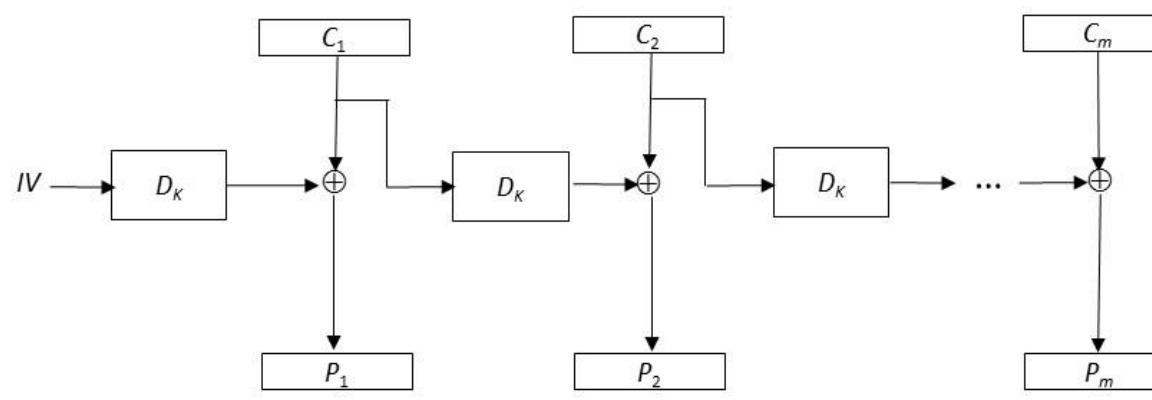
\includegraphics[width=126.00mm,height=109.89mm]{../../images/llm/page_041_img_01.png}%
\end{textblock*}

\end{document}
